% TeX file "application"

% Master thesis 
% Sven Jacobs
% Winter 2022, M.Sc. Economics, Bonn University
% Supervisor: Prof. Dr. Dominik Liebl


\section{Application} \label{sec:application}

To illustrate all the discussed steps in a bias-aware sharp RD analysis (identification, estimation, inference, validation),
we present an extensive application before the simulation study,
which then investigates inferential performance exclusively.
For the implementation of the application and simulation,
we particularly make use of the two \textsf{R} packages \texttt{rdrobust} by \citeauthor{Calonico_2019} and \texttt{RDHonest} by \citeauthor{Armstrong_2020}.
All materials (data, code, etc.) to replicate the results are available on GitHub:
\url{https://github.com/svjaco/master_thesis}

Our application is based on a prominent paper by \citeauthor{Ludwig_2007} (\citeyear{Ludwig_2007}, \citetitle{Ludwig_2007}).
In 1965 the U.S. launched the federal poverty alleviation program \enquote{Head Start}, targeted at poor children.
To receive funding, counties had to apply to a competitive selection process.
However, the federal government provided assistance to the 300 poorest counties to develop funding proposals.
\textcite[e.g.\ Figure I and II]{Ludwig_2007} document that this grant-writing assistance substantially increased Head Start participation and funding.
For example, 80 percent of the 300 treated counties received funding.
In their main analysis, \citeauthor{Ludwig_2007} used a sharp RD design to determine the local effect of grant-writing assistance
on child mortality due to causes the program's goal was to reduce.%
\footnote{Alternatively, we can think about the effect as an intent-to-treat effect of Head Start funding.} 
For estimation local linear regression is applied, but the bandwidth is chosen ad hoc, and their inference procedure ignores any potential bias.
Therefore, we review the original analysis and conduct validation checks, optimal bandwidth selection and bias-aware inference,
which have been developed after the paper's publication.

Table~\ref{tab:overview} provides a summary.
\begin{table}
	\centering
	\captionabove{Overview Head Start data set}
	\label{tab:overview}
	\resizebox{\textwidth}{!}{%
	\begin{tabular}{l l l}  
		\toprule 
		Assignment variable $(X)$ & County poverty rate in 1960        & Min:\,15.21 | Mean:\,36.73 | Max:\,81.57 \\
		Outcome $(Y)$             & Average mortality rate per 100000, & Min:\,0 | Mean:\,2.17 | Max:\,73.53 \\
		                          & Head Start related causes,         & \\
		                          & Ages 5--9, 1973--83                & \\		                          
		Cutoff $(c)$              & $X = 59.1984$                      & Poverty rate of 300th poorest county \\
		Treatment $(T)$           & Grant-writing assistance           & \\
		Additional covariates     & 14 (post: 4, prior: 10)            & See Table~\ref{tab:covariates} \\
		Number of observations    & 2781                               & Control: 2487, Treatment: 294 \\
		\bottomrule
	\end{tabular}}	
\end{table}
The assignment variable is the county poverty rate, obtained from the 1960 U.S. Census.
The outcome is the average mortality rate per 100000 for children of age 5--9, during 1973--83,
due to Head Start related causes (mainly anemia, meningitis and respiratory problems).
A county receives the treatment of grant-writing assistance when its poverty rate is above the cutoff 59.1984.
The raw data are plotted in Figure~\ref{fig:scatter}.
We have data on 2781 counties, with 294 of them above the poverty cutoff, receiving treatment.
We obtain more insights from the standard RD plot in Figure~\ref{fig:rdplot_Y}.
\begin{figure}
	\centering
	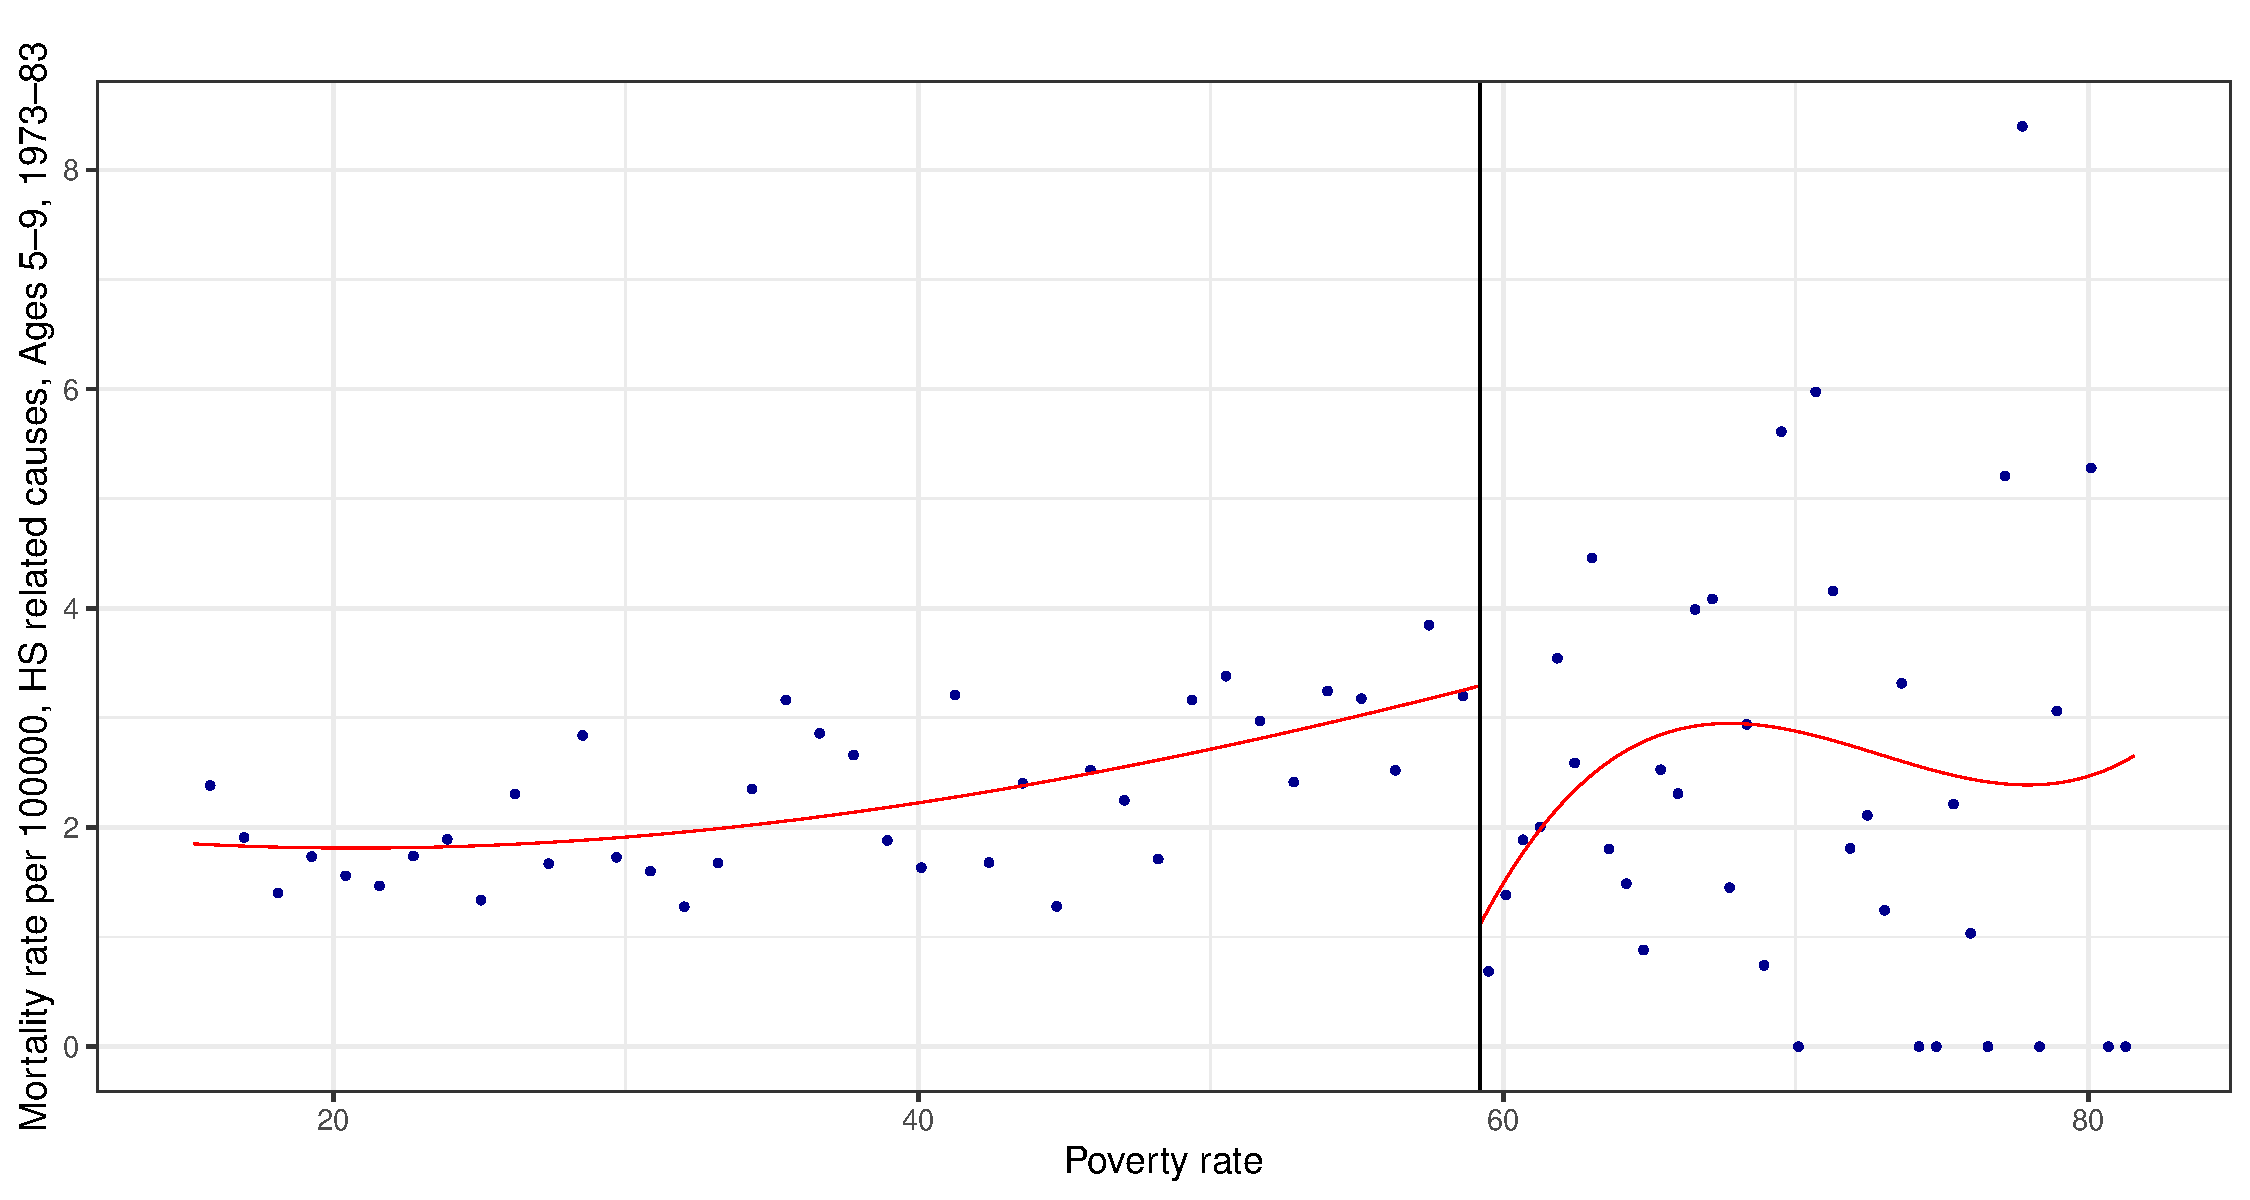
\includegraphics[width=\textwidth]{figure_04.pdf}
	\caption{Standard RD plot for the outcome of interest.
			 The dots depict the mean within each bin, where the bins are evenly spaced and their number is chosen to mimic the variance of the raw data (see \cite{Calonico_2015a}).
		 	 The solid red lines are third-order polynomial fits for control (left) and treated (right) counties separately.}
	\label{fig:rdplot_Y}
\end{figure}
The mortality rate increases nearly linearly in the poverty rate until the cutoff.
At the cutoff, the plot suggests a clearly visible downward discontinuity.
Afterwards, the mortality seems to rise nonlinearly.
Such a visualization provides valuable guidance, but can never replace a formal statistical treatment effect analysis
(remember the above mentioned problems of higher-order polynomial fitting).

The RD treatment effect $\tauSRD$ in the Head Start application is the ATE of receiving grant-writing assistance
on the Head Start (HS) related child mortality for a county with poverty rate in 1960 equal to 59.1984,
which reflects a very high poverty.
This effect can be identified with a sharp RD design if the continuity assumption holds.
That is, continuity (at the cutoff) of the expected potential mortality functions (with and without grant-writing assistance).
We have to be aware of two threats.
First, the cutoff might have been used in other federal social spending programs.
And second, the poverty rate might have been manipulated.
\citeauthor{Ludwig_2007} addressed the first concern and did not find any evidence for a discontinuity in other federal social spending at the Head Start cutoff.
Also, manipulation of the assignment variable can credibly been ruled out with the knowledge
that treatment was assigned in 1965 on the basis of official census information from 1960.
Nevertheless, we conduct the falsification tests from Section~\ref{sec:validation}.

The histogram of the poverty rate in Figure~\ref{fig:histogram} does not reveal any indication of sorting around the cutoff.
This is supported by a formal density-continuity-test, which clearly does not reject the null of continuity at the cutoff,
as illustrated in Figure~\ref{fig:rddensityplot}.
\begin{figure}
	\centering
	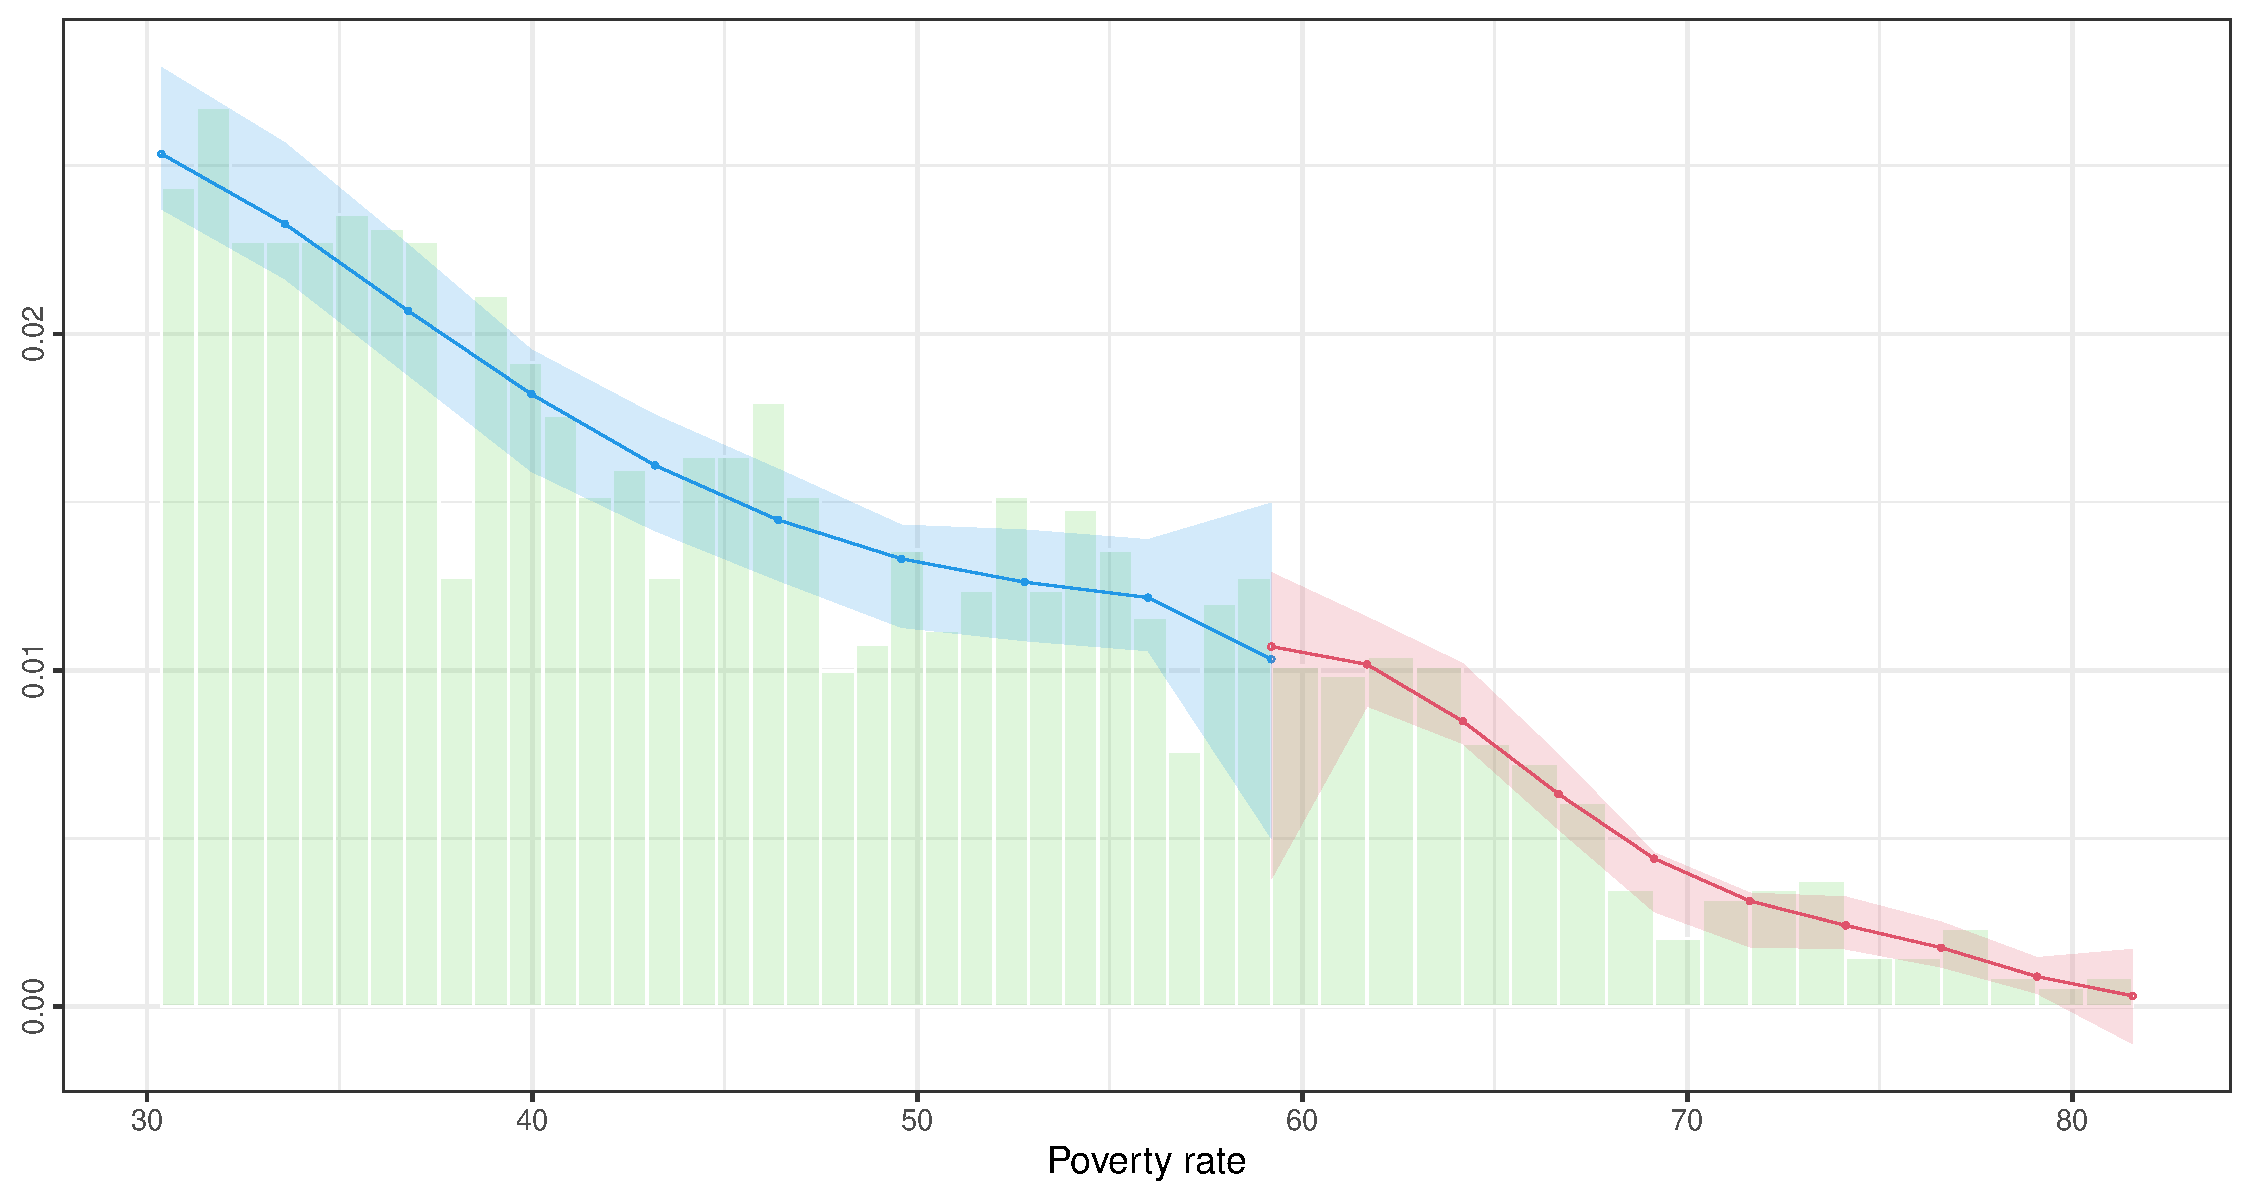
\includegraphics[width=\textwidth]{figure_05.pdf}
	\caption{Density-continuity-test for the poverty rate (assignment variable).
			 The density is estimated separately below (blue) and above (red) the cutoff,
		 	 using the local polynomial density estimator proposed by \textcite{Cattaneo_2020}.
	 	 	 The point estimates are non-centered, as the 95\% confidence intervals are robust bias-corrected.
 	 	 	 A histogram is added to the background.}
	\label{fig:rddensityplot}
\end{figure}
Next, we check whether statistically significant discontinuities can be found in variables where no treatment effect is expected.
For example, for other causes of death (mainly injuries) and the outcome of interest during the years 1959--64, before Head Start started.
For both variables we show the RD plot in Figure~\ref{fig:rdplots_cov}.
The plot for the pre-treatment HS related mortality does show a noticeable jump that requires further investigation.
Therefore, we perform a robust bias-corrected RD analysis and can debilitate the concern
(Figure~\ref{fig:llplot_Y_pre} combined with a robust $p$-value of 0.509 in Table~\ref{tab:covariates}).
The size of the jump in the RD plot is driven by the erratic behavior of the third-order polynomial at the cutoff.
Table~\ref{tab:covariates} reports the results of a separate RD analysis
(local linear estimation, triangular kernel, MSE-optimal bandwidth, RBC inference)
for each of the additional available covariates in the Head Start data set.
All 95\% robust confidence intervals contain zero.
For convenience the results are presented for the MSE-optimal instead of the CE-optimal bandwidth,
which might be a more suitable choice,
as we are mostly interested in inference here.
The conclusions, however, remain the same.
For completeness, we also report results from an RD analysis for placebo cutoffs (Table~\ref{tab:placebo_cutoffs})
and the donut-hole-approach (Table~\ref{tab:donut_holes}), as described at the end of Section~\ref{sec:validation}.
As a benchmark the results for $\tauhatSRD$ (i.e.\ effect at the true cutoff without excluded counties at the cutoff) are already included.
As expected, no significant effect at the artificial cutoffs occurs.
The donut-hole-analysis reveals that the results are somewhat sensitive to the degree of extrapolation at the cutoff.
Overall, the presented checks support the validity of the RD design. 

Let us now turn to the estimation of and inference for the effect of grant-writing assistance on the child mortality
(per 100000, ages 5--9, period 1973--83) due to HS related causes.
Our results are obtained for local linear estimation and the triangular kernel.
We consider the three bias-aware inference approaches from Section~\ref{sec:inference}:
undersmoothing, robust bias-correction, inflated critical value.
Standard errors are obtained via the nearest neighbor method.
The results are collected in Table~\ref{tab:HS_main} and visualized in Figure~\ref{fig:HS_main_plot}.
For the sake of comparison, the original findings from \textcite[Table~III]{Ludwig_2007} are reported as well.
Their bandwidths of $h^{\text{LM}}_1 = 9$ and $h^{\text{LM}}_2 = 18$ are ad hoc choices and
their inference procedure (bootstrapping the $t$-statistic) ignores potential bias.
Moreover, due to an error in the code, the applied kernel is the uniform kernel, and not (as stated) the triangular.
For the bandwidth of 9, \citeauthor{Ludwig_2007} report an estimate of $-1.895$, significant at the 5\% level.

\renewcommand{\arraystretch}{1.2}
\begin{table}[p]
	\centering
	\captionabove{Bias-aware analysis for the RD treatment effect in the Head Start application}
	\label{tab:HS_main}
	\resizebox{\textwidth}{!}{%
	\begin{tabular}{l l r c c c}  
		\toprule
		\multirow{2}[1]{*}{Approach} & \multicolumn{2}{c}{\multirow{2}[1]{*}{Bandwidth}} & \multirow{2}[1]{*}{RD estimate} & \multicolumn{2}{c}{Inference} \\
		\cmidrule(lr){5-6} 
		& & & & 95\% CI & $p$-value \\
		\midrule
		Undersmoothing                            & & & & & \\
		\quad -- By factor 2                      & $h^{\text{US}}_{1/2}$        & 3.457  & $-$3.428 & [$-$5.856, $-$1.001] & 0.006 \\
		\quad -- By factor 3                      & $h^{\text{US}}_{1/3}$        & 2.304  & $-$2.590 & [$-$5.488, 0.307]    & 0.080 \\
		Robust bias-correction                    & & & & & \\
		\quad -- MSE-optimal                      & $\hat{h}_{\text{MSE}}$       & 6.913  & $-$2.389 & [$-$5.426, $-$0.083] & 0.043 \\
		\quad -- CE-optimal                       & $\hat{h}_{\text{CE}}$        & 4.650  & $-$3.248 & [$-$6.092, $-$0.749] & 0.012 \\
		\quad -- MSE-optimal, incl. covariates    & $\tilde{h}_{\text{MSE}}$     & 7.115  & $-$2.445 & [$-$5.155, $-$0.339] & 0.025 \\
		\quad -- Ad hoc, \citeauthor{Ludwig_2007} & $h^{\text{LM}}_1$            & 9.000  & $-$2.182 & [$-$5.722, $-$0.350] & 0.027 \\
		\quad -- Ad hoc, \citeauthor{Ludwig_2007} & $h^{\text{LM}}_2$            & 18.000 & $-$1.681 & [$-$4.564, $-$0.101] & 0.040 \\
		\citeauthor{Armstrong_2020}               & & & & & \\
		\quad -- minimax MSE                      & $h^{\text{AK}}_{\text{MSE}}$ & 4.551  & $-$3.283 & [$-$6.039, $-$0.526] & 0.019 \\
		\quad -- Length-optimal                   & $h^{\text{AK}}_{\text{CIL}}$ & 4.670  & $-$3.239 & [$-$6.022, $-$0.456] & 0.022 \\
		\quad -- Ad hoc, \citeauthor{Ludwig_2007} & $h^{\text{LM}}_1$            & 9.000  & $-$2.182 & [$-$6.229, 1.866]    & 0.520 \\
		\quad -- Ad hoc, \citeauthor{Ludwig_2007} & $h^{\text{LM}}_2$            & 18.000 & $-$1.681 & [$-$11.700, 8.337]   & >0.9  \\
		\midrule
		\multicolumn{6}{l}{\citeauthor{Ludwig_2007} (bias ignored, uniform kernel)} \\
		\quad -- Ad hoc, \citeauthor{Ludwig_2007} & $h^{\text{LM}}_1$            & 9.000  & $-$1.895 &                      & 0.036 \\
		\quad -- Ad hoc, \citeauthor{Ludwig_2007} & $h^{\text{LM}}_2$            & 18.000 & $-$1.198 &                      & 0.081 \\                  
		\bottomrule \addlinespace[0.25ex]
		\multicolumn{6}{p{\dimexpr \textwidth+3\tabcolsep}}{\footnotesize \textit{Note}: Results are based on local linear estimation and the triangular kernel.
		The included additional covariates are all the variables from the Census 1960, as described in Table~\ref{tab:covariates}.
		For the approach by \citeauthor{Armstrong_2020}, the Hölder class and the global polynomial ROT $(M_{\text{ROT}}=0.299)$ are used.
		Due to an error in their code, the results from \textcite[Table~III]{Ludwig_2007} are obtained for the uniform kernel,
		and not (as reported) for the triangular.
		Their $p$-values are $t$-statistic-bootstrapped, ignoring potential bias.}
	\end{tabular}}	
\end{table}
\renewcommand{\arraystretch}{1.0}

\begin{figure}[p]
	\centering
	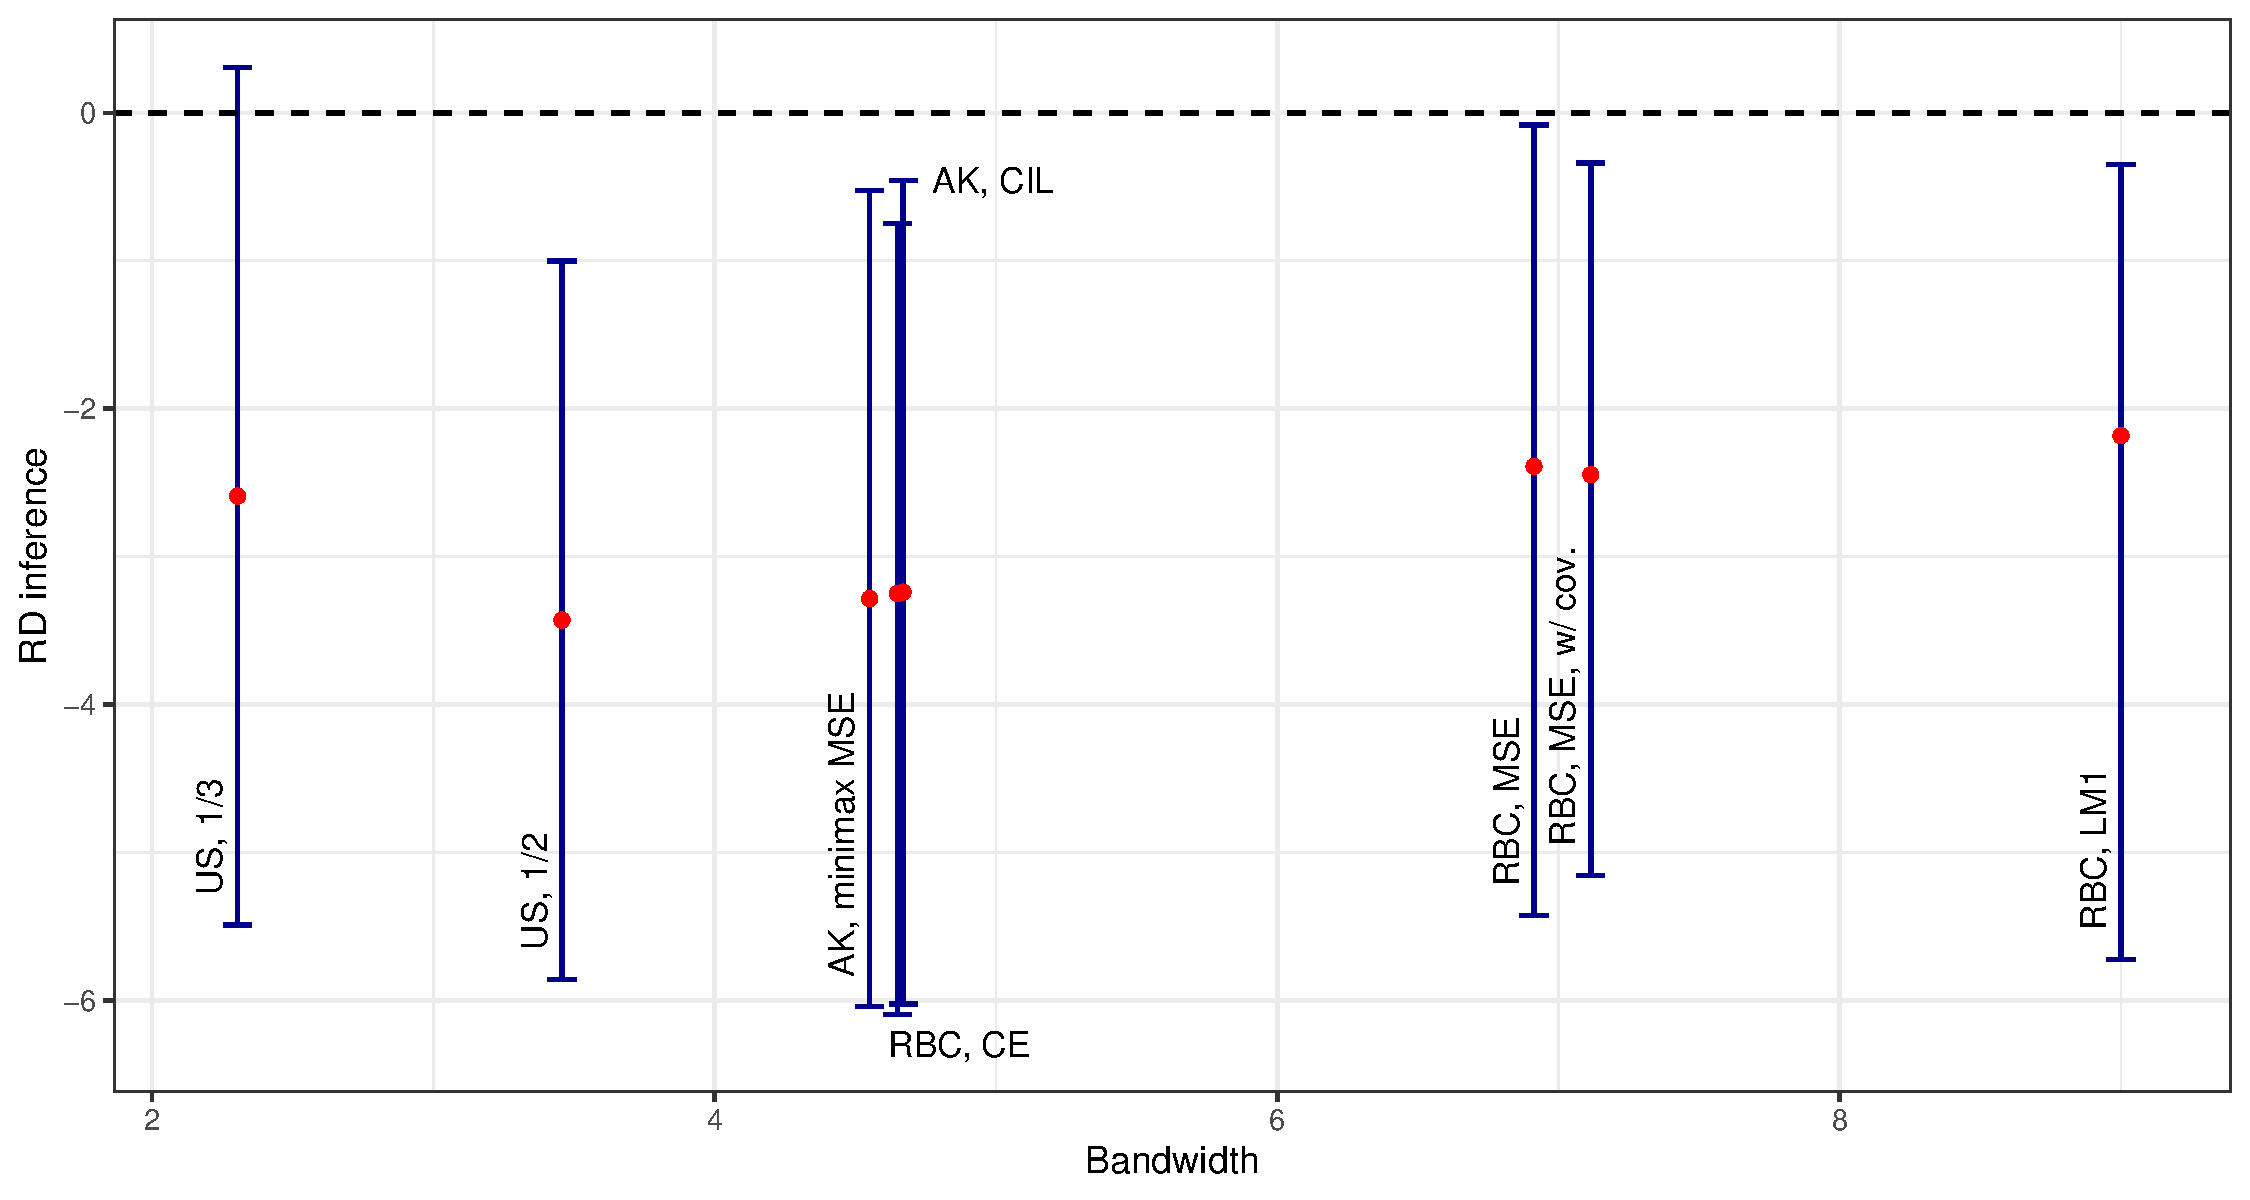
\includegraphics[width=\textwidth]{figure_06.pdf}
	\caption{Main results for the RD treatment effect in the Head Start application:
			 Point estimates and 95\% confidence intervals for the bias-aware inference approaches,
		 	 as presented in Table~\ref{tab:HS_main}.}
	\label{fig:HS_main_plot}
\end{figure}

We first compare with the RBC approach.
The estimated MSE-optimal bandwidth (using the plug-in selector of \cite{Calonico_2014}) is $\hat{h}_{\text{MSE}} = 6.913$,
leading to an estimated effect of $-2.389$ with robust $p$-value of 0.043.
Since the estimated untreated mortality at the cutoff for $\hat{h}_{\text{MSE}}$ is 3.585,
this is a large reduction of more than 60\%.
The MSE-optimal bandwidth suggests that the bandwidths of \citeauthor{Ludwig_2007} are too large (\enquote{oversmoothed}).
Including the nine predetermined variables from the U.S. Census 1960 (Table~\ref{tab:covariates})
showcases the potential gains from incorporating additional covariates.
The point estimate remains essentially the same, but the confidence interval is about 10\% tighter.
The CE-optimal bandwidth $\hat{h}_{\text{CE}} = 4.650$ is smaller and we obtain a larger (in magnitude) effect of $-3.248$.
To perform undersmoothing, we choose a bandwidth that is one half and one third of the MSE-optimal bandwidth, respectively.
Undersmoothing by 50\% yields the largest discontinuity out of all specifications ($-3.428$) and a relatively narrow confidence interval.
Estimating the bias for this undersmoothed bandwidth, however, indicates that bias is not negligible,
and the inference is too optimistic.
In contrast, for $h^{\text{US}}_{1/3}$ we get an estimate similar to the MSE-optimal one with a relatively wide confidence interval,
containing as the only one zero.
The third approach by \citeauthor{Armstrong_2020} requires the specification of the function class $\mathcal{G}$ and smoothness constant $M$ (Section~\ref{sec:AK}).
We choose the Hölder class (imposing smoothness away from the cutoff) and
the global polynomial rule of thumb to bound the second derivative of the conditional expectation function globally.
For these choices, the minimax bandwidth $h^{\text{AK}}_{\text{MSE}}$,
minimizing the maximum MSE of the local linear estimator over the specified class,
is 4.551 and thus 34\% smaller than $\hat{h}_{\text{MSE}}$.
The resulting RD estimate and confidence interval are close to the CE-optimal RBC results.
When the criterion is to optimize interval length while maintaining coverage, the bandwidth $h^{\text{AK}}_{\text{CIL}}$ is only slightly increased.

We conclude the following from the above presented.
Our results indicate that the bandwidths in the original paper are too large.
To theoretically justify these bandwidths within the approach of \citeauthor{Armstrong_2020},
the conditional expectation function has to be nearly linear (i.e.\ $M$ has to be substantially smaller).
This is not consistent with the data, when looking at the evolution of the average mortality rate in the treatment group in Figure~\ref{fig:rdplot_Y}.
Both, using the uniform kernel (estimate of $-1.895$ vs.\ $-2.182$ for the triangular kernel) and the oversmoothing
contribute to an understatement of the effect size.
Our bias-aware analysis yields larger confidence intervals (due to smaller bandwidths plus bias-awareness),
but at the same time larger treatment effects, leaving the original conclusion unchanged.
In summary, our analysis reaffirms the HS targeted mortality reducing effect of grant-writing assistance at the cutoff.

The application already indicates that how much to undersmooth is a delicate question,
and we might easily run into undercoverage if the bandwidth is still \enquote{too large}.
This is one of the points addressed in the upcoming simulation.  